\documentclass[11pt]{article}
\usepackage[margin=1in]{geometry}
\usepackage[T1]{fontenc}
\usepackage{float,amsmath,amssymb,booktabs,graphicx,enumitem,hyperref,caption}
\hypersetup{colorlinks=true,linkcolor=black,urlcolor=blue,citecolor=black}
\setlist{itemsep=2pt,topsep=3pt}
\captionsetup{font=small}
\setlength{\parskip}{4pt}
\setlength{\parindent}{0pt}

\title{\vspace{-1.6cm}Portfolio Selection with Limited Holdings on the NASDAQ-100\\
\large IEOR E4004 Milestone 4: Complete Optimization Model}
\author{Qianke Chen (qc2400) \quad Jieao Dai (jd4338) \quad Zicong Ou (zo2178)\\
Phonthakorn Phreuksa (pp3018) \quad Jenny Yao (jy3548)}
\date{\vspace{-0.6cm}}

\begin{document}
\maketitle

\textbf{Code and data:} \url{https://github.com/PhonthakornPhreuksa/ieor4004-group27e} \; (all paths are relative; see \texttt{README.md} to reproduce every number in this report).

\section{Changes Since Milestone 3}
A small equity fund or personal investor allocates a fixed budget across NASDAQ-100 stocks but can hold at most $K$ positions. We study how much the holdings limit costs in sample and how limited portfolios perform out of sample. This milestone implements the model in Python and Gurobi and runs it on the full data. Compared with Milestone 3 we made the following changes.

\begin{enumerate}[leftmargin=*]
\item \textbf{Baseline $\lambda$ fixed in advance} (CA feedback). We use $\lambda = 1$ for all baseline runs. This gives one unit of daily expected return and one unit of daily MAD equal weight, since both are in the same units. The grid $\lambda \in \{0, 0.25, 0.5, 1, 2, 5, 10\}$ is fixed now for Milestone 5. No value of $\lambda$ was chosen using test-period results.
\item \textbf{Buy-and-hold evaluation} (CA feedback). The portfolio is bought on the first test day and never rebalanced, so weights drift with prices (Section 5).
\item \textbf{Universe finalized.} 101 tickers were listed. Six have incomplete price histories (ALAB, CRWV, HONA, NBIS, SNDK, SPCX) and are excluded. We also drop GOOG because GOOG and GOOGL are two share classes of the same company. This leaves $n = 94$ stocks.
\item \textbf{Parameter values computed} (Section 3), and units and a feasibility note added to the formulation.
\end{enumerate}

\section{Final Formulation}
\textbf{Sets.} $N=\{1,\dots,94\}$ is the set of eligible stocks. $\mathcal{T}=\{1,\dots,T\}$ is the set of trading days in the estimation window, $T=501$ (October 2, 2023 to September 30, 2025).

\textbf{Parameters.}
\begin{itemize}[leftmargin=*]
\item $r_{it}$: simple daily return of stock $i$ on day $t$, from adjusted closes (decimal, 0.01 = 1\%).
\item $\mu_i = \frac{1}{T}\sum_t r_{it}$: sample mean daily return, our estimate of expected return (decimal per day).
\item $a_{it} = r_{it}-\mu_i$: centered daily return (decimal per day).
\item $K$: maximum number of holdings, $K\in\{5,10,20,50\}$, plus a run with no limit.
\item $\lambda = 1$: risk-aversion weight on MAD (unitless; baseline value).
\item $w_{\min}=0.01$, $w_{\max}=0.30$: minimum and maximum weight of a selected stock.
\end{itemize}

\textbf{Decision variables.}
\begin{itemize}[leftmargin=*]
\item $x_i \in [0,1]$ (continuous): fraction of the budget invested in stock $i$ (unitless).
\item $y_i \in \{0,1\}$ (binary): 1 if stock $i$ is held, 0 otherwise.
\item $d_t \ge 0$ (continuous): absolute deviation of the portfolio's daily return from its mean on day $t$ (decimal per day).
\end{itemize}

\textbf{Objective.}
\[
\max_{x,y,d}\quad \sum_{i\in N}\mu_i x_i \;-\; \frac{\lambda}{T}\sum_{t\in\mathcal{T}} d_t
\]
We maximize the estimated daily expected return of the portfolio minus $\lambda$ times its mean absolute deviation (MAD). MAD keeps the model linear and needs no covariance matrix \cite{konno}. Larger $\lambda$ gives a more cautious portfolio.

\textbf{Constraints.}
\begin{align}
&\textstyle\sum_{i\in N} x_i = 1 && \text{(1) invest the whole budget}\notag\\
&x_i \le w_{\max}\, y_i \quad \forall i && \text{(2) only held stocks get weight, at most 30\%}\notag\\
&x_i \ge w_{\min}\, y_i \quad \forall i && \text{(3) a held stock gets at least 1\%}\notag\\
&\textstyle\sum_{i\in N} y_i \le K && \text{(4) at most $K$ holdings}\notag\\
&d_t \ge \textstyle\sum_{i} a_{it}x_i,\quad d_t \ge -\textstyle\sum_{i} a_{it}x_i \quad \forall t && \text{(5)--(6) $d_t \ge |\text{portfolio return}_t - \text{its mean}|$}\notag\\
&x_i \ge 0,\; d_t \ge 0,\; y_i\in\{0,1\} && \text{(7) long-only, no leverage}\notag
\end{align}
Constraint (2) links the two decisions: a stock can receive money only if it is selected. Constraint (3) stops the model from holding tiny positions. Constraint (4) is the holdings limit we study. Because $d_t$ is penalized in the objective, it equals the absolute deviation at the optimum, so (5) and (6) turn the absolute value into linear constraints. \textbf{Feasibility note:} with $w_{\max}=30\%$, at least four stocks are needed to reach 100\%, so every $K\ge 4$ is feasible.

\textbf{Assumptions} (carried from Milestone 3, updated). A1 current constituents (survivorship and look-ahead bias). A2 incomplete histories excluded, GOOG dropped. A3 sample means estimate expected returns. A4 risk measured by MAD. A5 long-only, fully invested. A6 $K$, weight bounds and $\lambda$ are project choices. A7 no transaction costs, taxes or market impact. A8 adjusted closes include splits and dividends. A9 risk-free rate used only for evaluation; missing DGS3MO values (bond market holidays, 2 days in the test year) are filled with the previous day's rate. A10 buy-and-hold in the test year, no rebalancing.

\section{Data and Parameter Values}
Prices are adjusted daily closes from Yahoo Finance (via \texttt{yfinance}) for September 29, 2023 to September 30, 2026. Tickers come from the Nasdaq API, the benchmark is QQQ, and the risk-free rate is FRED series DGS3MO. Table~\ref{tab:params} summarizes the estimated parameters.

\begin{table}[H]
\centering\small
\caption{Estimated parameters on the estimation window (94 stocks, 501 days).}
\label{tab:params}
\begin{tabular}{lccc}
\toprule
 & Min & Median & Max\\
\midrule
Mean return $\mu_i$, annualized ($\times 252$) & $-49.9\%$ & $26.6\%$ & $174.2\%$\\
Daily MAD of stock $i$ & 0.75\% & 1.40\% & 4.34\%\\
\bottomrule
\end{tabular}

\vspace{2pt}
\footnotesize Highest $\mu_i$: APP, MSTR, RKLB, PLTR, NVDA. Lowest MAD: LIN, ADP, ROP, CSCO, PEP. Nine stocks have negative $\mu_i$.
\end{table}

\section{Implementation and First Results}
The model is written in Python with \texttt{gurobipy} (matrix API). It has 689 variables (94 continuous weights, 94 binaries, 501 deviations) and up to 1,192 constraints, which fits within Gurobi's free license. Each solve has a 300-second limit and a 0.01\% optimality gap target. All five runs reached proven optimality.

\begin{table}[H]
\centering\small
\caption{In-sample results at $\lambda=1$. Cost = (no-limit objective $-$ objective) / $|$no-limit objective$|$.}
\label{tab:insample}
\begin{tabular}{lcccccc}
\toprule
Portfolio & Holdings & Objective (daily) & Cost vs no limit & Exp.\ return (ann.) & Daily MAD & Runtime (s)\\
\midrule
$K=5$ & 5 & $-0.00434$ & 24.0\% & 36.7\% & 0.58\% & 100.2\\
$K=10$ & 10 & $-0.00370$ & 5.8\% & 33.6\% & 0.50\% & 60.8\\
$K=20$ & 20 & $-0.00351$ & 0.25\% & 33.5\% & 0.48\% & 3.8\\
$K=50$ & 25 & $-0.00350$ & 0\% & 32.7\% & 0.48\% & 1.1\\
No limit & 25 & $-0.00350$ & -- & 32.7\% & 0.48\% & 1.4\\
\bottomrule
\end{tabular}
\end{table}

\textbf{Cost} is how much lower the objective is than in the no-limit portfolio, in percent. Objective values are negative because, at $\lambda=1$, daily MAD is larger than daily expected return; only the comparison between portfolios matters. The in-sample cost of simplicity falls quickly. Holding 20 stocks costs only 0.25\% of the objective, 10 stocks cost 5.8\%, and 5 stocks cost 24\%. The fewer stocks allowed, the harder the problem: $K=5$ took about 100 seconds, while the no-limit run took about one second.

\subsection*{Sanity checks}
\begin{itemize}[leftmargin=*]
\item \textbf{Constraints hold.} For every solution, code checks that weights sum to 1, every held weight is between 1\% and 30\%, no unselected stock has weight, and holdings do not exceed $K$. All checks pass.
\item \textbf{Objective recomputed independently.} Recomputing expected return minus $\lambda\cdot$MAD directly from the weights matches Gurobi's objective, which confirms that the $d_t$ linearization equals the true absolute deviation.
\item \textbf{The cost moves in the right direction.} Allowing more holdings never makes the objective worse. With no limit the model holds 25 stocks, so $K=50$ does not bind and gives exactly the same portfolio as no limit, as expected.
\item \textbf{The integer program adds value.} A shortcut that keeps the $K$ largest weights from the no-limit portfolio and re-optimizes on them is worse than the MILP by 8.2\% ($K=5$), 4.3\% ($K=10$) and 0.2\% ($K=20$). Simply trimming a continuous solution does not give the best limited portfolio, which matches the experience at GMO \cite{bertsimas}.
\item \textbf{Holdings make economic sense.} With $\lambda=1$ the model favors low-volatility stocks. The $K=5$ portfolio holds AEP (30\%), WMT (27\%), ORLY (21\%), TTWO (13\%) and NVDA (9\%). Utilities and consumer staples reduce MAD, and NVDA adds return.
\item \textbf{Extreme $\lambda$ behaves as theory predicts.} With $\lambda=0$ the model ignores risk and holds only 4 stocks, the minimum needed under the 30\% cap, with an expected return of 160\% a year. As $\lambda$ rises the no-limit portfolio spreads out, from 14 stocks at $\lambda=0.25$ to 28 at $\lambda\ge 5$. So $K=5$ and $K=10$ bind for every $\lambda \ge 0.25$, and $K=20$ binds for $\lambda \ge 1$. Our research question is meaningful in this range, and the baseline $\lambda=1$ lies inside it.
\end{itemize}

\section{First Out-of-Sample Look (Buy-and-Hold)}
Following the CA's feedback, each portfolio is bought on October 1, 2025 at its optimal weights and held to September 30, 2026 without rebalancing. The equal-weight portfolio uses the same rule. Sharpe ratios use the DGS3MO rate.

\begin{table}[H]
\centering\small
\caption{Out-of-sample results, October 1, 2025 to September 30, 2026 (251 trading days).}
\label{tab:oos}
\begin{tabular}{lcccc}
\toprule
Portfolio & Total return & Annual volatility & Sharpe ratio & Max drawdown\\
\midrule
$K=5$ & $-1.7\%$ & 12.8\% & $-0.37$ & $-11.8\%$\\
$K=10$ & 3.5\% & 10.4\% & 0.02 & $-10.4\%$\\
$K=20$ & 2.1\% & 9.6\% & $-0.14$ & $-7.3\%$\\
No limit ($=K=50$) & 3.1\% & 9.3\% & $-0.04$ & $-6.5\%$\\
Equal weight (94 stocks) & 45.2\% & 22.6\% & 1.60 & $-12.7\%$\\
QQQ & 23.8\% & 20.0\% & 0.98 & $-12.0\%$\\
\bottomrule
\end{tabular}
\end{table}

\begin{figure}[H]
\centering
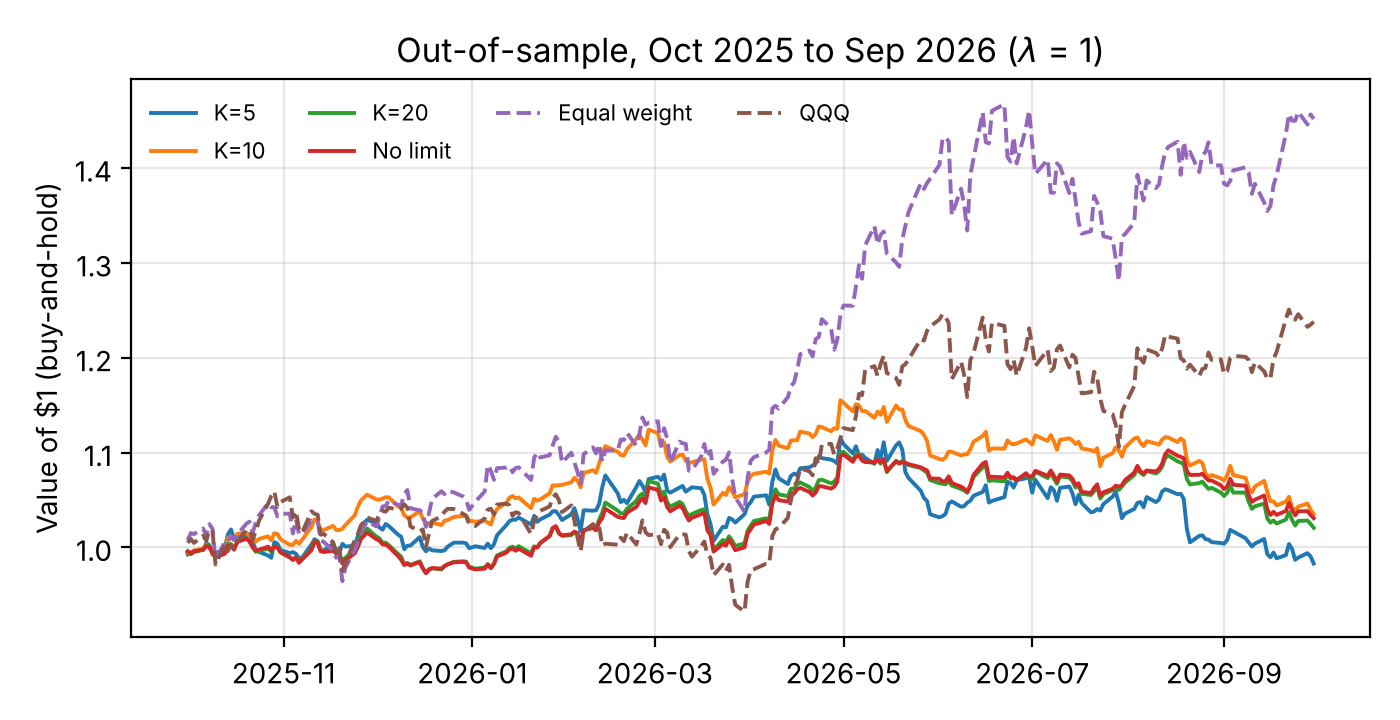
\includegraphics[width=0.85\textwidth]{../results/oos_value.png}
\caption{Value of \$1 invested on October 1, 2025. $K=50$ is hidden because it equals the no-limit portfolio.}
\end{figure}

\textbf{What this shows.} The optimized portfolios did what the objective asked. They had about half the volatility of QQQ and smaller drawdowns, and more holdings gave a smoother path. But in a strong rising market they missed most of the gain. This is a first look at a single $\lambda$, not a conclusion. Two points need care. First, the equal-weight benchmark is likely flattered by survivorship bias, because today's index members are partly the stocks that did well (A1). Second, the in-sample means are noisy \cite{michaud}, which is why we fix $\lambda$ in advance rather than tune it on the test year.

\section{Next Steps for Milestone 5}
\begin{itemize}[leftmargin=*]
\item Run the full $\lambda$ grid for every $K$ and plot the in-sample cost of simplicity and out-of-sample performance against $K$.
\item Vary the weight bounds ($w_{\max}$ of 20\% and 40\%) and the train/test split, including rolling windows, to test whether results hold beyond one year.
\item Report the trade-off between runtime and $K$, since small $K$ is the hardest case for the solver.
\end{itemize}

\section*{AI Use Disclosure}
We used two AI assistants as writing and modeling aids while preparing this report. Kimi helped us brainstorm formulations, check our algebra and derivations, and polish the wording. Claude helped us write the Python and Gurobi code, download the data from the sources listed in Section 3, and draft parts of the text. All modeling choices, including the universe, weight bounds, values of $K$, and the baseline $\lambda$, were decided by the group, and the group reviewed and re-ran the code and verified the results.

\begin{thebibliography}{9}\small
\bibitem{konno} Konno, H., and Yamazaki, H. (1991). Mean-absolute deviation portfolio optimization model and its applications to Tokyo stock market. \emph{Management Science}, 37(5), 519--531.
\bibitem{michaud} Michaud, R. O. (1989). The Markowitz optimization enigma: Is ``optimized'' optimal? \emph{Financial Analysts Journal}, 45(1), 31--42.
\bibitem{bertsimas} Bertsimas, D., Darnell, C., and Soucy, R. (1999). Portfolio construction through mixed-integer programming at Grantham, Mayo, Van Otterloo and Company. \emph{Interfaces}, 29(1), 49--66.
\end{thebibliography}
\end{document}
